\section{Versuchsaufbau/-durchführung}
Ziel des verwendeten Aufbaus ist die Photoluminesz-Emission verschiedener Nanokristalle in Abhängigkeit
von der Anregungswellenlänge, der Intensität und der Polarisation spektral zu untersuchen.
Hierzu wird eine Anordnung nach Abbildung~\ref{fig: aufbau} verwendet. Die einzelnen Komponenten
im Strahlengang sollen nun näher beschrieben werden.

\begin{figure}
  \centering
  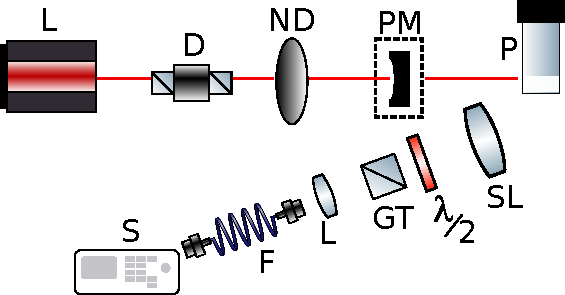
\includegraphics[width = 0.6\textwidth]{pics/setup.pdf}
  \caption{Schematische Darstellung des verwendeten Aufbaus. Komponenten: Laser (L, hier nur schematisch rot dargestellt), Optische Diode (D), Neutraldichtefilter (ND),
  dichroischer Spiegel (DM), optionales Leitsungsmessgerät (PM), Probe (P), Sammellinse (SL), $\lambda / 2$-Plättchen, Glan-Taylor-Prisma (GT), Filter zur Unterdrückung
  der Laserwellenlänge (F), Linse (L), optische Fiber (OF), Spektrometer (S).}
  \label{fig: aufbau}
\end{figure}

Zunächst wird als Anregungslichtquelle eine Laserdiode mit $\lambda = \SI{405}{\nano\meter}$ verwendet.
Die Pumpstromstärke wird während aller Messungen auf den maximalen Wert von etwa $\SI{150}{\milli\ampere}$ eingestellt.
Das ausgesandte Licht passiert eine optische Diode, die Rückkopplungseffekte minimieren soll.
Anschließend folgt ein einstellbarer Neutraldichtefilter, mit dem die auf einen Maximalwert eingestellte Laserleistung
verringert werden kann. Die Leistung lässt sich mit einem optional einsetzbaren Leistungsmessgerät bestimmen.
Dahinter passiert das Licht einen
dichroischen Spiegel, der nur Licht für Licht unterhalb von
$\lambda = \SI{425}{\nano\meter}$ transparent ist.
Anschließend gelangt das Laserlicht auf die Probe. Hierbei handelt es sich um Nanokristalle in Pulverform, die sich in
einem durchsichtigen Kunststoffgefäß befinden. Unter einem Winkel von $\SI{20}{\degree}$ zur optischen Achse wird der
Detektionspfad installiert. Das gestreute Licht wird zunächst mit einer Sammelinse eingefagen. Zur Überprüfung auf eine
mögliche Polarisation der Photoluminsz wird eine Kombination aus $\lambda / 2$-Plättchen und
Glan-Taylor-Prisma verwendet. Ein optischer Filter unterdrückt die Wellenlänge des Lasers.
Abschließend wird das Licht mit einer Linse auf den Eingang einer Faser fokussiert, die mit einem
Spektrometer verbunden ist. Mit einer Computer-Steuerung können Spektren aufgenommen werden. Die Aufnahmezeit beträgt
$\SI{1}{\second}$.

Es werden Photolumineszenzspektren von drei verschiedenen Proben aufgenommen. Anschließend wird eine Abhängigkeit von der
Leistung und von der Polarisation überprüft. Abschließend werden andere Anregungswellenlängen verwendet. Hierzu wird
eine Weißlicht-Quelle eingesetzt, aus der mit optischen Filtern die Wellenlängen
$\SI{470}{\nano\meter}$ und $\SI{520}{\nano\meter}$ extrahiert werden. Hier wird zusätzlich zur Fokussierung vor die Probe eine
Linse eingesetzt.
